\documentclass[a4paper, 12pt]{article}

\def\languages{french, english}

%%%%%%%%%%%%%%%%%%% Libraries

\input{include/libraries/bibliography.tex}
\input{./include/libraries/default.tex}
\input{./include/libraries/figures.tex}
\input{./include/libraries/mathematics.tex}
\input{./include/libraries/units.tex}

%%%%%%%%%%%%%%%%%%% Bibliography

\addbibresource{resources/bib/ref.bib}

%%%%%%%%%%%%%%%%%%% Titlepage

\def\logopath{./resources/pdf/logo.pdf}
\def\toptitle{University of Liège}
\title{Project 3 - Supervised classification}
\def\subtitle{\textsc{MATH2021-1} - High-dimensional data analysis}
%\def\authorhead{}
\author{
Yann \textsc{Claes} (s161317)\\
Gaspard \textsc{Lambrechts} (s161826)\\
François \textsc{Rozet} (s161024)\\
}
%\def\rightauthorhead{}
%\def\rightauthor{}
\def\context{MSc in Data science and engineering}
\date{Academic year 2019-2020}

%%%%%%%%%%%%%%%%%%%

\usepackage{mhchem}
\usepackage{wrapfig}

%%%%%%%%%%%%%%%%%%%

\begin{document}
	\input{./include/titlepages/default.tex}
	\pagenumbering{roman}
	\section*{Data}
	
	The \num{500} measures of pollutant concentrations and atmospheric conditions from the Shunyi station used in project 1 and 2 having a very unbalanced binary indicator (\texttt{rain}), it has been decided to restart from the \num{35 000} measures made at this station, and work on the mean daily pollutant concentrations. From this new data, the binary variable will be defined as "exceeding the weighted WHO\footnote{World Health Organization} recommendations for \emph{at least} one of the pollutants". This binary variable will be detailed below.
	
	Taking the average of the \num{24} (one per hour) concentrations for each day, and considering only the rows without missingness (complete case analysis), the data is now composed of \num{1461} observations and \num{13} variables, described in the table \ref{tab:variables}.
	
	\begin{table}[h]
	    \centering
	    \begin{tabular}{r|l}
	         year & year \\ \hline 
	         month & float month\footnotemark \\ \hline
	         PM2.5 & daily mean PM2.5 concentration \\ \hline
	         PM10 & daily mean PM10 concentration \\ \hline
	         \ce{SO2} & daily mean \ce{SO2} concentration \\ \hline
	         \ce{NO2} & daily mean \ce{NO2} concentration \\ \hline
	         \ce{O3} & daily mean \ce{O3} concentration \\ \hline
	         temp & daily mean temperature \\ \hline
	         pres & daily mean pressure \\ \hline
	         dewp & daily mean dew point \\ \hline
	         rain & daily mean rain \\ \hline
	         wspd & daily mean wind speed \\ \hline
	         wdir & daily dominant wind direction\footnotemark
	    \end{tabular}
	    \caption{Variables of the new dataset}
	    \label{tab:variables}
	\end{table}
	\footnotetext{Mapping of each day (at noon) of the year to a float between $0$ and $12$.}
	\footnotetext{The most common wind direction, with frequency of appearance weighted by the wind speed. Expressed as an angle (\si{\radian}) oriented counterclockwise from east direction.}
	
	Hence, \texttt{day} has been removed because it is contained in \texttt{month} and \texttt{CO} has been removed because no WHO recommendations are made for this pollutant. All other variables except \texttt{wdir} have been aggregated by mean of means. \texttt{wdir} has been taken as kind of the most frequent wind direction over the day, taking the wind speed into account. This data is saved in the file \texttt{products/csv/data.csv}.
	
	Averaging over the days has consequences since all peaks will be smoothed, but for the needs of this project (predicting if one of the daily mean pollutant concentration will surpass a given value), it does not seem too problematic to work on the daily mean of each variable. Furthermore, as a sensor is often down for a certain number of time (and thus a series of consecutive measures), some of the daily means will be measured on only on very few measures, being certainly biased. It will be considered as acceptable given the low missing rate of the data.
	
	\subsection*{Binarization of the data}
	
	For the following questions, the pollutant concentrations will all be replaced by one single binary indicator: \emph{\og{}Does one of the pollutant mean concentrations overpass the WHO recommendations over a day weighted by some margin ?\fg{}}, represented by the variable \texttt{alert}.
	
	The WHO recommendations can be found in Table \ref{tab:who}. It has been chosen to use the maximum mean concentration over \SI{8}{\hour} as the daily mean \ce{O3} concentration threshold (as no data is provided for one day). For other pollutants, we used the actual one-day threshold given by the WHO.
	
	The binary variable has been defined as 
	\begin{center}
	\texttt{alert = any(mean\_pollutant\_concentrations > margins * recommendations)}
	\end{center}
	
	where the \texttt{margins} have been artificially tuned to \texttt{[3 3 1 1 1]} and the recommendations taken to \texttt{[25 50 20 200 100]} as said above. We justify this arbitrary margins by the fact that the particle matter (PM) concentrations are around 80\% of the time above the WHO recommendations at Shunyi station in Beijing, it can thus seem not useful to alert for a danger each time that the PM concentrations are above these thresholds, but alert when these concentrations reach a less frequent but more dangerous threshold, such as three times the WHO recommendation.

	\begin{table}[h]
	    \centering
	    \begin{tabular}{|c|c|c|c|c|}
	    \hline
	         \multirow{2}{*}{Pollutant} & \multicolumn{4}{c|}{Max. mean exposition over} \\ \cline{2-5}
	         & \SI{1}{y} & \SI{1}{\day} & \SI{8}{\hour} & \SI{10}{\minute} \\ \hline\hline
	         PM2.5 & \SI{10}{\micro\gram\per\meter\cubed} & \SI{25}{\micro\gram\per\meter\cubed} &  &  \\
	         PM10 & \SI{20}{\micro\gram\per\meter\cubed} & \SI{50}{\micro\gram\per\meter\cubed} &  &  \\
	         \ce{SO2} &  & \SI{20}{\micro\gram\per\meter\cubed} &  & \SI{500}{\micro\gram\per\meter\cubed} \\
	         \ce{NO2} & \SI{40}{\micro\gram\per\meter\cubed} & \SI{200}{\micro\gram\per\meter\cubed} &  &  \\
	         \ce{O3} &  &  & \SI{100}{\micro\gram\per\meter\cubed} &  \\ \hline
	    \end{tabular}
	    \caption{Recommendation for maximum mean pollutant exposition over a certain period}
	    \label{tab:who}
	\end{table}
	
	\section*{Feasibility of the classification}
	
	On the one hand, from the analysis conducted in part 1 of the project, we know that there exists a strong correlation structure between the pollutant concentrations and the atmospheric conditions (\texttt{temp}, \texttt{dewp}, \texttt{pres}). Our binary variable being based on the pollutant concentrations, achieving a classification based on all the other variables (including the atmospheric ones) seems promising.
	
	On the other hand, the PCA analysis conducted in part 2 of the project indicated that the total variance of the dataset was mainly contained in two independent (by construction) principal components (gathering \SI{68}{\percent} of the total variance), the first one being roughly composed of the pollutant variables, the second one being roughly composed of the atmospheric variables. We thus see that a non negligible part of what we would like to be in our explanatory variables (atmospheric variables) is uncorrelated with what has constituted, after binarization, our dependent variable (pollutant variables). 
	
	Also, from project 1, we know that the \texttt{year} doesn't have much of an influence on other variables. Therefore, it shouldn't have any significant influence over the \texttt{alert} variable.
	
	\newpage
	
	\pagenumbering{arabic}
	
	\section{Classification using the logistic regression model}
	
	\subsection{Finding a logistic regression model}
	Using as explanatory variables all the remaining quantitative variables (i.e. \texttt{year}, \texttt{month}, \texttt{temp}, \texttt{pres}, \texttt{dewp}, \texttt{rain}, \texttt{wspd} and \texttt{wdir}), we built a first logistic regression model to predict the binary value of \texttt{alert}. This yielded the coefficients summary of Table \ref{tab:first_model_coeff}.
	
	\begin{table}[h]
	    \centering
	    \begin{tabular}{|c|c|c|c|c|c|}
    	    \cline{2-5}
    	    \multicolumn{1}{c|}{} & Estimate &  Std. Error &  $z$ value & Pr$(>\abs{z})$ & \multicolumn{1}{c}{} \\ \hline
    	    Intercept & \num{426.09986} & \num{110.89546} & \num{3.842} & \num{0.000122} & *** \\ \hline
    	    year & \num{-0.17430} & \num{0.05517} & \num{-3.159} & \num{0.001581} & ** \\ \hline
    	    month & \num{-0.12790} & \num{0.02113} & \num{-6.053} & \num{1.42e-09} & *** \\ \hline
    	    temp & \num{-0.24125} & \num{0.02152} & \num{-11.210} & $<$ \num{2e-16} & *** \\ \hline
    	    pres & \num{-0.07032} & \num{0.01289} & \num{-5.456} & \num{4.88e-08} & *** \\ \hline
    	    dewp & \num{0.15057} & \num{0.01633} & \num{9.220} & $<$ \num{2e-16}  & *** \\ \hline
    	    rain & \num{-1.17392} & \num{0.32761} & \num{-3.583} & \num{0.000339} & *** \\ \hline
    	    wspd & \num{-0.51387} & \num{0.11119} & \num{-4.622} & \num{3.81e-06} & *** \\ \hline
    	    wdir & \num{0.32787} & \num{0.03944} & \num{8.312} & $<$ \num{2e-16}  & *** \\ \hline
	    \end{tabular}
	    \caption{Coefficients summary of the full logistic model}
	    \label{tab:first_model_coeff}
	\end{table}
	
	The corresponding AIC value is equal to \num{1572.6}.
	
	\begin{wrapfigure}{R}{0.4\textwidth}
	    \vspace{-1.5em}
	    \centering
	    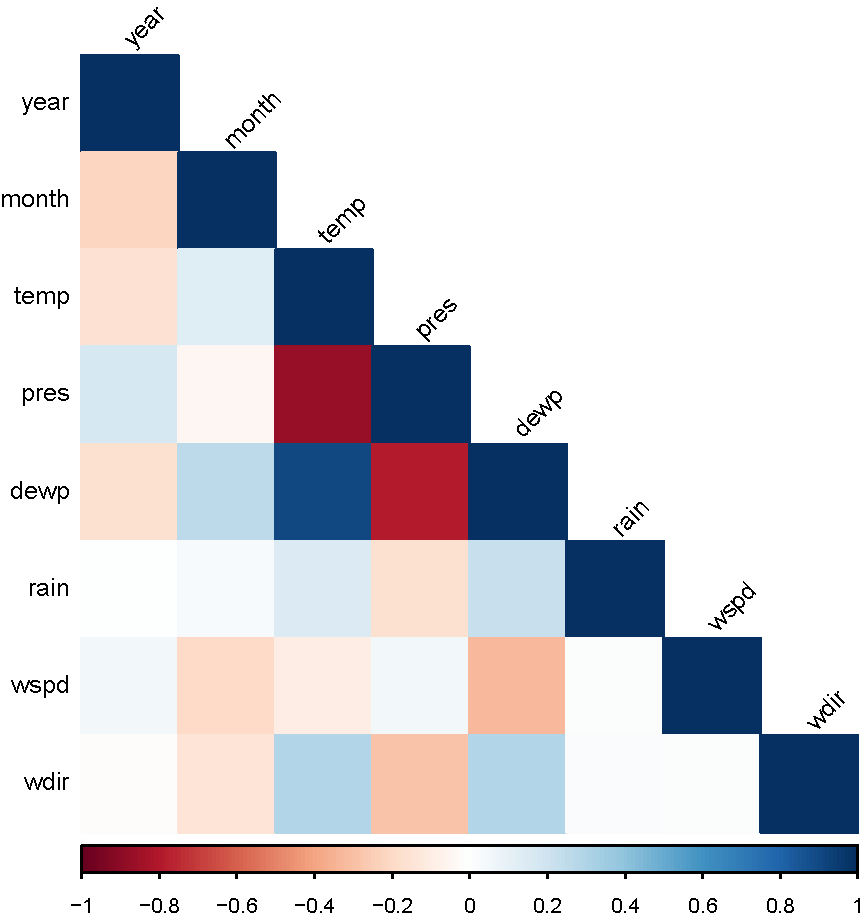
\includegraphics[width=0.4\textwidth]{resources/pdf/correlation_plot.pdf}
	    \caption{Correlation plot of the explanatory variables}
	    \label{fig:corrplot}
	    \vspace{-1.5em}
	\end{wrapfigure}
	
	From the summary, we see that all explanatory variables seem to have an important influence on the logistic model. The last column (Pr$(>\abs{z})$) represents the probability that a coefficient that should be zero has a higher absolute value than the estimated coefficient. This value being extremely low for all coefficients, we can reject the null hypothesis of having a zero coefficient.
	
	We then decided to draw a correlation plot between the explanatory variables, in order to spot a potential multicollinearity between them, leading to Figure \ref{fig:corrplot}. From this plot, we can see that \texttt{temp}, \texttt{pres} and \texttt{dewp} are strongly correlated, which is not a surprise if we keep in mind the correlation analysis that was conducted in the first project.
	
	To emphasize this behavior, we computed the associated VIF scores, which can be found in Table \ref{tab:vif_scores}.
	
	\begin{table}[h]
	    \centering
	    \begin{tabular}{cccccccc}
	        year & month & temp & pres & dewp & rain & wspd & wdir \\
	        \hline
	        \num{1.091} & \num{1.405} & \num{14.553} & \num{4.316} & \num{12.649} & \num{1.166} & \num{1.462} & \num{1.232}
	    \end{tabular}
	    \caption{VIF scores of the explanatory variables of the full model}
	    \label{tab:vif_scores}
	\end{table}

	From these VIF scores, we can see that the temperature and dew point have very big VIF scores compared to all other variables, and that the pressure has a greater VIF score than the other explanatory variables (except \texttt{temp} and \texttt{dewp}). We should thus keep these scores in mind when looking at the estimated coefficients of Table \ref{tab:first_model_coeff}, as they might lead to a wrong insight of the interpretability of the influence of the explanatory variables due to this multicollinearity behavior. In order to check whether a major issue is introduced, we constructed three different models where each one contained all the other variables and either \texttt{temp}, \texttt{pres} or \texttt{dewp}. Then, we compared the coefficients of these three variables (in terms of sign and absolute value), leading to Table \ref{tab:pres_dewp_temp_coeff}.
	
	\begin{table}[h]
	    \centering
	    \begin{tabular}{|c|c|c|c|}
	        \cline{2-4}
    	    \multicolumn{1}{c|}{} & \texttt{temp} & \texttt{pres} & \texttt{dewp} \\ \hline
    	    Full model & -0.24125 & -0.07032 & 0.15057 \\ \hline
    	    Reduced models & -0.023704 & -0.0001157 & -0.0005504 \\ \hline
	    \end{tabular}
	    \caption{Coefficients of \texttt{temp}, \texttt{pres} and \texttt{dewp}}
	    \label{tab:pres_dewp_temp_coeff}
	\end{table}
	From this table, we can observe that the parameters differ a lot from the full model to the reduced models, emphasizing the impact of multicolinearity.
	
	To get rid of this problem, we decided to replace these three variables by the first principal component of the data restricted to these three variables, and to build a model with this principal component as well as the remaining variables. This yielded the coefficients summary of Table
	\ref{tab:modified_model_coeff}, with an AIC of 1717.
	
	\begin{table}[h]
	    \centering
	    \begin{tabular}{|c|c|c|c|c|c|}
    	    \cline{2-5}
    	    \multicolumn{1}{c|}{} & Estimate &  Std. Error &  $z$ value & Pr$(>\abs{z})$ & \multicolumn{1}{c}{} \\ \hline
    	    Intercept & 317.876628 & 103.695226 &  3.065 & 0.00217 & ** \\ \hline
    	    year & -0.157033 &  0.051459 & -3.052 & 0.00228 & ** \\ \hline
    	    month &  -0.081628 & 0.018506 & -4.411 & 1.03e-05 & *** \\ \hline
    	    rain & -0.231231 & 0.261069 & -0.886  &0.37577 & \\ \hline
    	    wspd & -1.071795 & 0.103444 & -10.361 & < 2e-16 & *** \\ \hline
    	    wdir & 0.321574 & 0.036226 & 8.877 & < 2e-16  & *** \\ \hline
    	    PC1 & -0.004691 &  0.003484 & -1.346  & 0.17817 &  \\ \hline
	    \end{tabular}
	    \caption{Coefficients summary of the modified logistic model}
	    \label{tab:modified_model_coeff}
	\end{table}
	
	Deriving this modified model does not come with a gain of interpretability of the model.
	
	In order to select the optimal set of explanatory variables, we decided to perform a backward AIC selection of the variables using the function \texttt{stepAIC}. This resulted in the optimal model corresponding to the model where the variable \texttt{rain} is removed, as the AIC is minimized in that case. We also performed a forward variable selection, which yielded the same results\footnote{These results can be found in the source code \texttt{logistic\_regression.R}.}.
	
	\paragraph{Interpretation of the model}
	From the coefficients of Table \ref{tab:modified_model_coeff}, we can see that the principal component resuming the three colinear variables will have very little impact on the classification rule. This result was suggested in the preliminary discussion about the feasibility of the prediction. Most of the other variables (except \texttt{rain} which is removed from the model) have a negative coefficient, while only the intercept and \texttt{wdir} have positive coefficients. For example, the bigger the wind speed, the smaller the probability of success, and thus the smaller the probability of having a pollutant concentration surpassing the recommendations. 
	
    We have
    \begin{align*}
        \mathrm{logit}(\pi) & = 317.88 - 0.157 \texttt{year} - 0.082\texttt{month} - 1.072\texttt{wspd} + 0.321\texttt{wdir} - 0.005\texttt{PC1}\\
        \pi & = \frac{\exp(317.88 - 0.157 \texttt{year} - 0.082 \texttt{month} - \ldots)}{1 + \exp(317.88 - 0.157 \texttt{year} - 0.082\texttt{month} - \ldots)} 
    \end{align*}
	The classification rule is
	\begin{equation*}
	    \pi > 0.5
	\end{equation*}
	
	\paragraph{Fitted values and residuals}
	As far as the fitted values are concerned, we get the boxplot of Figure \ref{fig:boxplot_fitted_values}. The mean value of the fitted values is equal to \num{0.515647}, which is quite close to the median, and \SI{75}{\percent} of the fitted values lie between \num{0.386870} and \num{0.674243}. We can thus observe that the model does not predict extreme values but rather moderate values for the probability of success, which corroborates what has been concluded in the correlation structure of project 1.
	\begin{figure}[h]
        \centering
        \begin{subfigure}{0.48\textwidth}
            \includegraphics[width = \textwidth]{resources/pdf/boxplots_fitted_values.pdf}
            \caption{Boxplot of the fitted values}
            \label{fig:boxplot_fitted_values}
        \end{subfigure}
        \hspace{0.5em}
        \begin{subfigure}{0.48\textwidth}
            \includegraphics[width=\textwidth]{resources/pdf/boxplots_residuals.pdf}
            \caption{Boxplot of the Pearson residuals}
            \label{fig:boxplot_pearson_residuals}
        \end{subfigure}
    \end{figure}
	The computed residuals correspond to the Pearson residuals, and are summarized in the boxplot of Figure \ref{fig:boxplot_pearson_residuals}. The mean of these residuals is equal to \num{0.009266}, meaning that residuals are, on average, close to zero, and thus that the fitted model is quite good on the data we provided it with.
	
	The error rate of the predictions is equal to \num{0.3100996}, which means that the model does not seem to be too bad at determining whether a pollutant concentration will surpass the recommendations or not. We should however keep in mind that this rate was computed on the same dataset as the one used to build the model. It is thus normal that the error rate is not too high. 
	
	\subsection{Performance of the classification model}
    As a reminder, the optimal model is composed of the following variables: \texttt{year}, \texttt{month}, \texttt{wspd}, \texttt{wdir} and \texttt{PC1}. The leave-one-out cross-validation yielded the confusion matrix of Table \ref{tab:leave_one_out}.
    \begin{table}[h]
    \centering
    \begin{tabular}{cc|cc}
                                &   & \multicolumn{2}{c}{Estimated} \\
                                &   & 0                 & 1               \\ \hline
    \multirow{2}{*}{True} & 0 & 400               & 281             \\
                                & 1 & 440               & 285             
    \end{tabular}
    \caption{Confusion matrix for the leave-one-out technique.}
    \label{tab:leave_one_out}
    \end{table}
    From this confusion matrix, we can compute the total error rate which is around \SI{50}{\percent}. This rate is much higher than the one obtained previously, which shows that the prediction model is maybe not as good as expected. 
    
    The sensitivity and specificity values have also been computed, and are respectively equal to \num{0.3931034} and \num{0.5873715}. This means that the model fails at predicting a surpassing pollutant concentration around six times out of ten, and correctly predicts the non-surpassing behavior about \SI{60}{\percent} of the time.
    
    To get more insight about the performance of the classification model, we decided to draw the ROC curve corresponding to the leave-one-out technique, yielding Figure \ref{fig:ROC_curve}.
    
    \begin{figure}[h]
        \centering
        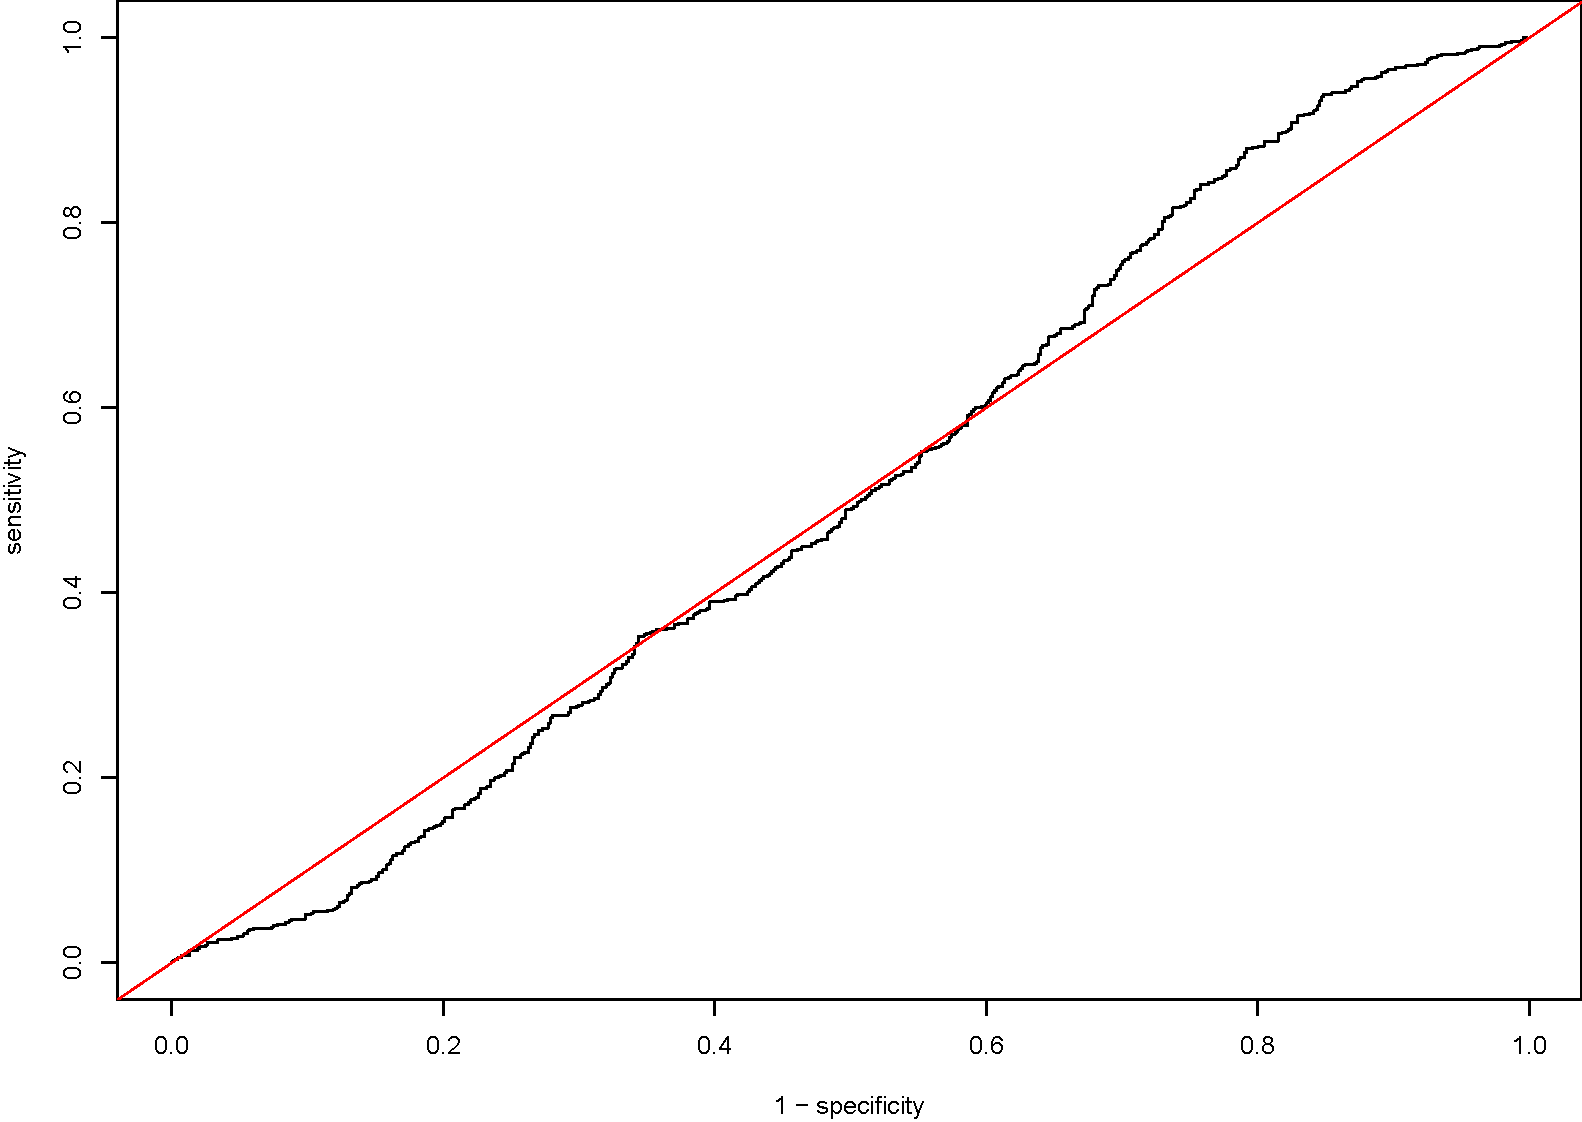
\includegraphics[width=0.65\textwidth]{resources/pdf/ROCCurve.pdf}
        \caption{ROC curve of the leave-one-out technique}
        \label{fig:ROC_curve}
    \end{figure}
    
    We can indeed see that the ROC curve follows a curve quite similar to the random model, \textit{i.e.} the model predicting 0 or 1 with equal probabilities. To corroborate this observation, we computed the area under the ROC curve, which is equal to $0.5053643$.
    
    \newpage
    
    \section{Classification based on LDA scores}
    
    \subsection{Canonical variable and scores}
    
    Initially using all the quantitative variables (centered and scaled), the LDA procedure resulted in the most discriminant direction described by the coefficients of the Table \ref{tab:lda_coef}. 
    
    \begin{table}[h]
	    \centering
	    \begin{tabular}{cccccccc}
	        year & month & temp & pres & dewp & rain & wspd & wdir \\
	        \hline
	        \num{-0.180} & \num{-0.375} & \num{-2.234} & \num{-0.605} & \num{1.721} & \num{-0.201} & \num{-0.330} & \num{0.516}
	    \end{tabular}
	    \caption{LDA canonical projection coefficients}
	    \label{tab:lda_coef}
	\end{table}
	
	As a result, the canonical variable expression is 
	\begin{align*}
	    Z_1 = -\num{0.180} \texttt{year} - \num{0.375} \texttt{month} - \num{2.234} \texttt{temp} - \num{0.605} \texttt{pres} + \ldots
	\end{align*}
	The scores are then obtained by projection, i.e. by evaluating $Z_1$ for each row of the dataset.
	
	\begin{figure}[h]
        \centering
        \begin{subfigure}{0.48\textwidth}
            \includegraphics[width = \textwidth]{resources/pdf/lda_full_scatter.pdf}
            \caption{Scatter plots of the scores w.r.t \texttt{alert}}
        \end{subfigure}
        \hspace{0.5em}
        \begin{subfigure}{0.48\textwidth}
            \includegraphics[width=\textwidth]{resources/pdf/lda_full_boxplot.pdf}
            \caption{Boxplots of the scores w.r.t \texttt{alert}}
        \end{subfigure}
    \end{figure}
    
    As one can see, the LDA procedure didn't succeed greatly at separating both distributions, which is corroborated by its quite low discriminant power $\gamma_1 = \num{0.2406}$. This result means that both distributions overlap a lot within the $\Rl^p$ space, it is therefore not possible to completely separate them. The reason could simply be that the quantitative variables are not sufficiently linked to the constructed \texttt{alert} values.
    
    \subsection{Suppressing less discriminant variables}
    
    In table \ref{tab:lda_coef}, one can observe that the variables \texttt{year} and \texttt{rain} are the one with the lowest influence on the canonical variable and, therefore, the score. As far as \texttt{year} is concerned, this observation sticks with the preliminary analysis. For \texttt{rain}, we can see a parallel with the previous section (Logistic regression) where \texttt{rain} was removed from the dataset to increase the AIC.
    
    Indeed, by looking at Table \ref{tab:leave_one_out_gamma}, we can see that removing either \texttt{year} or \texttt{rain} doesn't significantly reduces the discriminant power of the method, conversely to any other variables.
    
    \begin{table}[h]
	    \centering
	    \begin{tabular}{c|cccccccc}
	        out & year & month & temp & pres & dewp & rain & wspd & wdir \\
	        \hline
	        $\gamma$ & \num{0.2351} & \num{0.2206} & \num{0.1527} & \num{0.2242} & \num{0.1872} & \num{0.2340} & \num{0.2278} & \num{0.1992}
	    \end{tabular}
	    \caption{Leave-one-variable-out discriminant powers}
	    \label{tab:leave_one_out_gamma}
	\end{table}
    
    By removing both, the cardinal variable becomes 
    \begin{align*}
	    Z_1' = - \num{0.326} \texttt{month} - \num{2.137} \texttt{temp} - \num{0.642} \texttt{pres} + \num{1.555} \texttt{dewp} - \num{0.389} \texttt{wspd} + \num{0.543} \texttt{wdir}
	\end{align*}
	and its associated discriminating power decreases to \num{0.2281}.
	
	\subsection{Classification using the scores}
	
	Using the simplified model (without \texttt{year} and \texttt{rain}), we computed, as before, the scores $z$ of each individual $x$. The perfect classification rule would be to assign to an individual the group with the highest probability knowing the individual. However, in practice, it is not possible to compute exactly this probability.
	
	Yet, we can approximate the result of such rule by selecting the group with greatest posterior probability\footnote{If the prior probability was (very) unbalanced we should have considered it in the computations, fortunately it is not the case (we are almost perfectly balanced). Also, potential misclassification cost haven't been considered.} that the individual belongs in it. Moreover, under the normality assumption and the assumption of \emph{homoscedasticity} of the covariance matrices in each group, one can show that finding the greater posterior probability is the same as finding the group whose center (mean) is the closest to the individual.
	
	
	
	Therefore if we wish to classify the rows based on their scores (obtained previously) using that rule we have
	$$\text{group} = 1\rbk{\abs{z - \bar{z}_1} \leq \abs{z - \bar{z}_0}}$$
	where $\bar{z}_1$ and $\bar{z}_0$ are respectively the mean scores of the group $1$ and $0$.
	
	Applying such rule on our dataset yields table \ref{tab:conf_mat}.
	
	\begin{table}[h]
        \centering
        \begin{tabular}{cc|cc}
                                    &   & \multicolumn{2}{c}{Estimated} \\
                                    &   & 0                 & 1         \\ \hline
              \multirow{2}{*}{True} & 0 & 477               & 204       \\
                                    & 1 & 206               & 519             
        \end{tabular}
        \caption{Confusion matrix of leave-one-out LDA classification.}
        \label{tab:conf_mat}
    \end{table}
    
    Surprisingly, the results aren't that bad with \SI{70.8}{\percent} of correct classification !
    
    \subsection{Homoscedasticity assumption}
    
    As stated in the previous section, the classification rule has been partially derived from the assumption of \emph{homoscedasticity} of the covariance matrices in each group. Yet, this assumption has still to be validated, i.e. to prove that the variability of the quantitative variables is (more or less) the same in each group.
    
    First of all, we computed the scores' variance in both groups : \num{1.101} for the group $0$ and \num{0.905} for the group $1$. These are fairly close. We also computed the covariance matrices in both groups.
    
    \begin{figure}[h]
        \centering
        \begin{subfigure}{0.48\textwidth}
            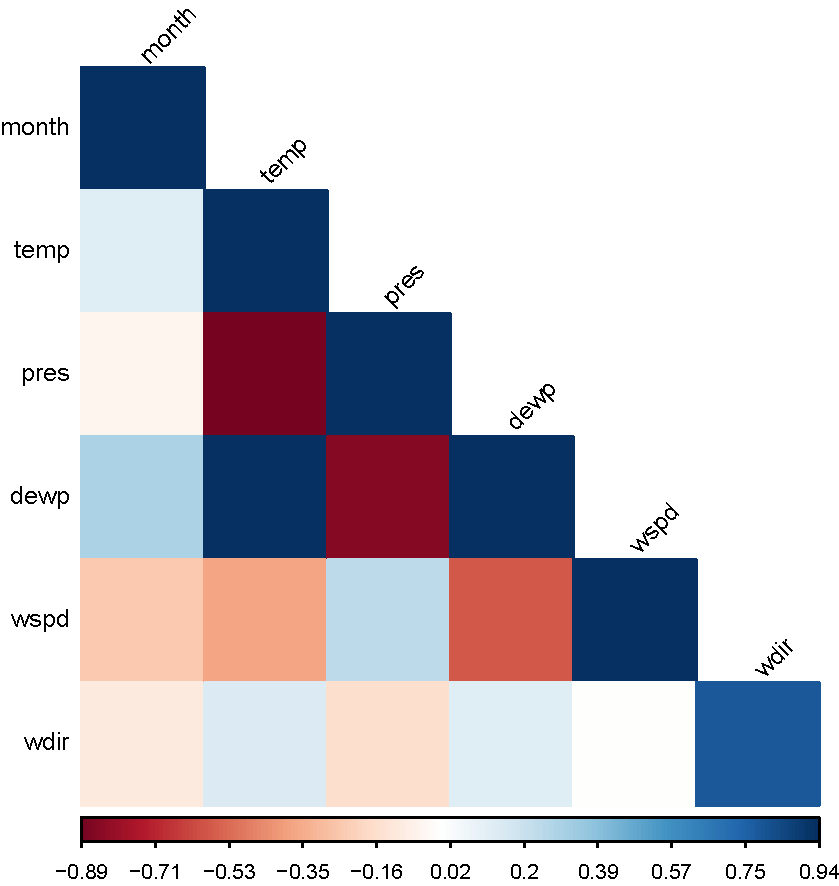
\includegraphics[width = \textwidth]{resources/pdf/cov_group_false.pdf}
            \caption{Covariance matrix of group $0$}
        \end{subfigure}
        \hspace{0.5em}
        \begin{subfigure}{0.48\textwidth}
            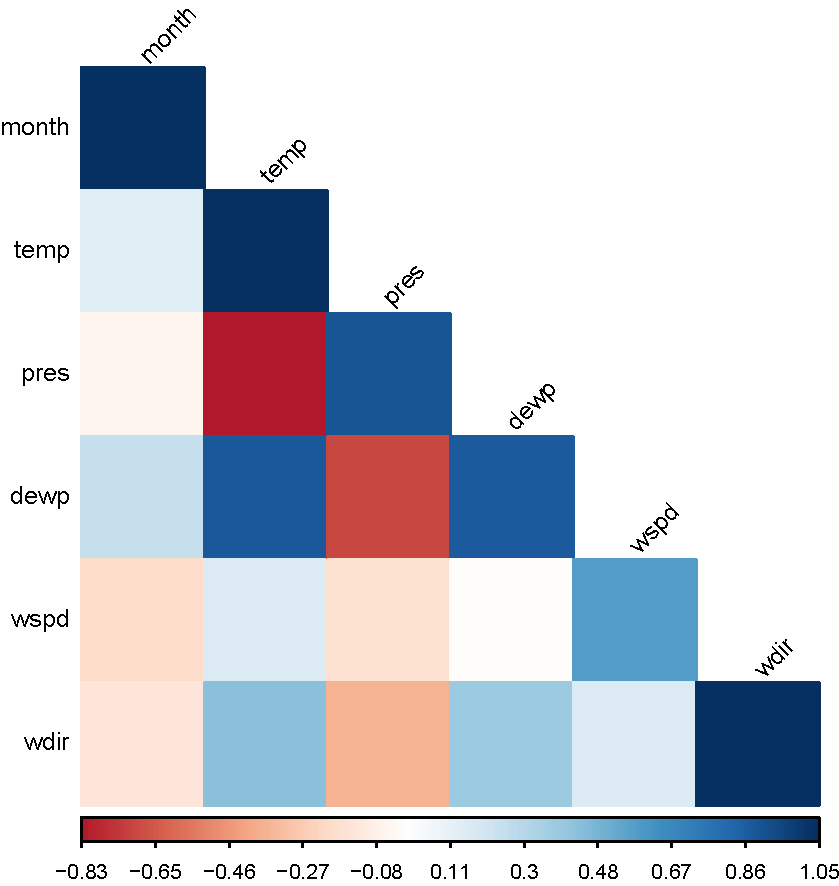
\includegraphics[width=\textwidth]{resources/pdf/cov_group_true.pdf}
            \caption{Covariance matrix of group $1$}
        \end{subfigure}
    \end{figure}
    
    As we can see, both matrices aren't totally similar, yet not dissimilar enough to invalidate the homoscedasticity assumption.
    
\end{document}
